\documentclass[12pt]{article}
\usepackage[margin=0.5in]{geometry}
\usepackage[margin=0.5in]{caption}



\usepackage{graphicx}
%\usepackage{amsmath}
%\usepackage{amsfonts}
%\usepackage{amssymb}
%\usepackage{amsthm}
%\usepackage{multicol}
%\usepackage{algorithms}
%\usepackage{showkeys}

%\newtheorem{Definition}{Definition}
%\newtheorem{Lemma}{Lemma}
%\newtheorem{Corollary}{Corollary}
%\newtheorem{Proposition}{Proposition}
%\newtheorem{Theorem}{Theorem}
%\newtheorem{Conjecture}{Conjecture}
%\newtheorem{Remark}{Remark}
%\newtheorem{question}{Question}
%\newtheorem{QaA}[question]{Q\&A}


\begin{document}

\title{Angry Ants: Final Report}
%\date{\today}
\author{Jasmin Uribe and Yunhao Xu}
\maketitle
\abstract Analyzing the motion and behavior of social insects requires tracking many individuals over time. Automated tracking is unreliable and inefficient. Ants frequently interact with each other which can cause the algorithm to begin tracking a different ant. The high density of ants being observed also increases the complexity of automated tracking. The authors of \cite{Joy12} use a ``citizen scientist" model where volunteers track ants. A representative trajectory is then extracted for each ant using Frechet average and median trajectory. The authors propose a global approach in which all ant trajectories are considered simultaneously. In this paper we construct a trajectory graph for data collected by citizen scientists and explore a global greedy approach for extracting representative trajectories.  We also explore the sensitivity of this global approach to changes in input parameters using generated data. We measure the average variance in pixels of each representative trajectory from the ground truth. Our results demonstrate that for the collected data, the global greedy approach works well; matching if not out-performing the automated solution. We also demonstrate that the global greedy algorithm is sensitive to probability of user error and the clustering threshold.

%We also propose an alternative method of determining trajectories based on DNA shot-gun sequencing.
\section{Introduction}
\indent Biologists are exploring the social dynamics of ant colonies in order to better understand social organization in animal groups. In studying ant colonies, data is collected by tracking ant motion and interactions. Following each individual ant manually is impractical and time consuming. Automated tracking algorithms are unreliable and inefficient. Ants interact frequently by meeting, touching or crawling over each other. This makes tracking an individual ant difficult for an automated system. 
\indent The authors of \cite{Joy12} have created a system that allows volunteers to track ants in videos in order to apply the ``citizen-scientist" model to this problem. Users build a trajectory by clicking on a specified ant at every time step. Once enough data is collected an `average' trajectory is extracted using a ``local" approach: a representative trajectory for each ant is computed using either a Frechet average or median trajectory. The authors then compare these representative trajectories to an existing automated ant tracking system and to the `ground truth'. See Fig. \ref{fig:ALocal}.

\begin{figure}
\centering
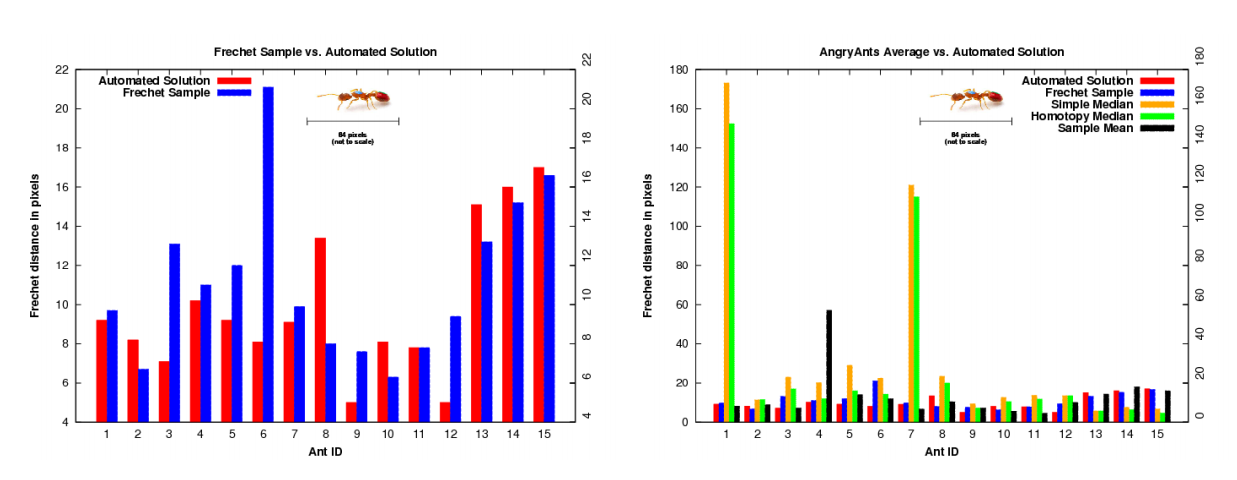
\includegraphics[width = 6.2in]{AntsJU.png}
\caption{Frechet distance between trajectories and `ground truth' \cite{Joy12}}
\label{fig:ALocal}
\end{figure}

\indent A complementary ``global" approach is described briefly in \cite{Joy12}. In this approach trajectories for all $k$ ants are considered simultaneously. Citizen scientists often mistakenly switch from tracking one ant to tracking another when two or more ants intersect. The global approach is motivated by this phenomenon; an ant trajectory could contain valid portions of another ants path. See Fig. \ref{fig:AGraph}.

\begin{figure}[h!]
\centering
\includegraphics[width = 3.7in]{Antgraph.png}
\caption{Trajectory graph $G$ \cite{Joy12}}
\label{fig:AGraph}
\end{figure}

%\indent In the unweighted case, the $x$-weight is proportional to the number of users who believe that ant $x$ moved through that edge between time $t_i$ and $t_{i+1}$. In order to find the $k$ edge-disjoint paths that begin at the source, end at the sink and cover all edges of $G$, a network flow instance is created. The difficulty here is the solution of the network flow may choose an inappropriate sequence of edges as the trajectory for a given ant. Thus the goal becomes compute a network flow with $k$ paths of different colors with the extra constraints so that each path is `feasible' and `optimal'. These extra constraints mean that the problem is neither the standard network flow problem nor a multi-commodity flow problem.


\indent Some work has been done on the global approach, in \cite{Cruz13}, several algorithms, both local and global, were compared using collected data. Here, we explore the representative trajectories extracted by a global greedy algorithm. We then compare the resulting trajectories to the `ground truth' and measure the average variance. In order to further test the quality of the algorithms, we generate pseudo-random ant paths, simulate user data, then extract representative trajectories and compare to the actual ant paths. We explore the sensitivity of the global greedy algorithm to input parameters.
%Finally we propose a new algorithm to extract ant trajectories based on DNA shot-gun sequencing.

\indent This paper is organized as follows. Related work is described in Section 2. Section 4 contains the graph generating algorithms. Section 5 details the collection and generation of data. The experiments are described in section 7. We discuss results and describe future work in sections 8 and 9.

\section{Related Work}
Object tracking is defined as the problem of estimating the trajectories of certain objects in an image as they move around a defined space. Other relevant data such as orientation, shape and area of an object may be collected as well. Tracking objects is complex in many ways due to noise in the images, complex object motion, illumination changes and loss of the third dimension in 2D images, to name a few. Many approaches have been proposed for this problem, each addressing a slightly different issue.\\
\indent  \cite{Yilmaz06}  by Yilmaz {\it et al.} provides a survey of tracking methods grouped into broad categories. The purpose of the paper is to provide a library of tracking algorithms allowing readers to select the most appropriate based on their needs. They discuss the importance of object representation, object appearance, feature selection, object detection, background subtraction, and image segmentation. Different types of object tracking- point tracking, kernel tracking and silhouette tracking- are also discussed, as well as which algorithms are best suited to each. \\
\indent The authors of \cite{Maitra09} present a method for tracking bees that uses static and adaptive appearance templates as well as ``geometry-constrained resampling of particles for handling appearance change." Tracking bees, much like tracking ants, is difficult since the objects are all very similar and the appearance of an object can change over time. With bees, the placement of the wings, the orientation of the bee, and the uneven lighting affect how the bee will appear in the image. Appearance templates provide a more complete description of the appearance, making the algorithm more sensitive to specific features of the bee. The added resampling step improves the prediction of head and thorax orientation. Together these modifications improve tracking when compared to a particle filtering based tracking with Gaussian modeling of appearance.\\
\indent In a more recent paper, the authors of \cite{Fletcher11} present a method for tracking multiple ants. They ``prevent drifts by maximizing the coverage of foreground pixels at a global scale" and ``improve speed by reducing Markov chain length through dynamically changing the target proposal distribution for perturbed ant selection." They used the fact that in many cases the number of ants being tracked remained constant for a certain period of time combined with the assumption that all ant pixels are tracked to reduce the algorithm erroneously switching from one ant path to another. They also increased efficiency by using a ``variable target proposal distribution." Not all ants move at every time step, so instead of using a fixed distribution they dynamically vary the distribution based on the level of expected motion. These changes improve both accuracy and speed.\\
\indent One of the major problems with automatic tracking methods is drifting, which occurs when the tracker loses the object it is tracking. In 2012, \cite{Poff12} addressed this problem by enabling a user to examine a fraction of the entire sequence for validating and correcting mis-trackings. Frames containing drifts were identified ``based on the amount of un-tracked foreground pixels;" this modification improved automated tracking by 25\%.\\
\indent Markov chain Monte Carlo based particle filters were used by \cite{Zuria08} to effectively deal with interacting targets whose behavior is dependent on its interactions with others. They propose a model that maintains the identity of the objects throughout an interaction in order to reduce drifting. The algorithm is based on the assumption that certain objects do not behave independently, but rather an encounter between two objects can result in very different behavior. This paper demonstrates how ``a Markov random field motion prior, built on the fly at each time step, can adequately model these interactions."\\
\indent Once the data has been collected, using an automated tracking algorithm or otherwise, it must then be analyzed. There are two general approaches: the local approach, in which we consider individual trajectories, and the global approach, in which we consider all trajectories. Some research has been done on determining an average path given a data set of many paths and much work has been done on averaging polygonal paths. In \cite{Morris}, they present an approach for finding recreational trails using aerial images and maps. They assume the two end points of the trail are given, then find the most likely trail between the points. They estimate the likelihood that an observed piece of an image is on the trail using three different models. They then integrate this approach with a more global approach by noting that pieces of a trail must link up to connect the start point with the end point. \\
\indent The authors of \cite{Buchin10} ``establish criteria that a `median trajectory' should meet" then present methods of computing said median. Two of the properties of a median trajectory are that any point, $p$, on the median must also lie on an input trajectory and the minimum number of distinct trajectories $p$ must cross to reach the unbounded face is $\frac{m+1}{2}$, where $m$ is the number of input trajectories. The authors of \cite{Joy12} use this definition of a median trajectory in one of the local approaches.\\
\indent When considering the local approach, it is necessary to define a measure of how close one path is to another. In many papers the Frechet distance is used. In \cite{Driemel10} a practical approximation algorithm is presented for the Frechet distance between two polygonal curves. The Frechet distance can be thought of as the maximum distance a point on the first curve has to travel as this curve is being continuously deformed into the second curve. A new class of curves for which the Frechet distance can be approximated quickly is introduced.\\
\indent The authors of `Matching Planar Maps' by {\it Alt et al.} \cite{Alt03} present an algorithm ``for measuring the similarity patterns of line segments in the plane." They consider a polygonal curve and an embedded graph with line segment edges. The goal is to find a path in the graph that minimizes the Frechet distance between the path and the curve. This idea is modified in \cite{Buchin09} where exact algorithms are determined for partial curve matching using Frechet distance. Here, they measured partial similarity between curves. The goal was to maximize the total length of sub-curves that are close to each other. They present a polynomial-time exact algorithm for computing this maximum.\\
%\indent \cite{Blum2008ant} presents a version of sequencing by hybridization using an ant colony optimization algorithm. Applies the basic ACO algorithm within a "multilevel framework", which reduces a problem to smaller instances by successive coarsening until a stopping criteria is reached. This paper also includes a list of papers detailing other approaches to SBH.\\
%\indent \cite{Li2008map} describes a DNA sequence mapping algorithm that is well suited to efficiently aligning large amounts of short reads (30 - 40 base pairs) to a reference genome. Also described is a method to determine the confidence that such mapping was performed correctly. The source code is freely available.\\
\indent Currently there is experimental work being done on a linear programming approach to solve the global network flow problem \cite{Cruz13}. In this case, weights are assigned to each edge for each ant. These weights should add up to 1. The goal is to maximize the $(weight)*(cost)$ over all edges and all ants.  For each vertex, the sum of incoming weights of each ant should equal the sum of outgoing weights of that particular ant. The conjuncture is that for each edge the weight of one ant will be 1 and the weight of all other ants will be 0. Most recently a counterexample has been found that demonstrates a case in which an integer solution will never be reached. 

\section{Our Contribution}
We explore the global greedy algorithm of extracting a representative trajectory for each ant. We demonstrate that this algorithm is sensitive to changes in the probability of user error and the clustering threshold. \\
We define a {\it trajectory} as a sequence of ordered triples $(t_1, x_1, y_1), (t_2, x_2, y_2),..., (t_N, x_N, y_N)$ where $x_i$ is the x-coordinate and $y_i$ is the y-coordinate of an ant at time $t_i$. We connect these points with straight lines, assuming ants move at a constant speed between time steps. Let $\tau_1,...,\tau_n$ a collection of trajectories. We assume each trajectory tracks one of $k$ ants and each ant is tracked at least once. We assume each trajectory has the same number of points. We also assume the starting point of each trajectory is certain. Given this collection of trajectories we wish to compute a representative trajectory for each ant. We define a representative trajectory as the most likely path taken by each ant. \\
We compute this representative trajectory using a global greedy algorithm. We use a hybrid clustering algorithm to first create a global graph then use a greedy algorithm to determine the most likely path for each ant. Recent work has determined that this problem is NP-hard, but our global greedy algorithm performs well for collected data when compared to the automated solution. \\
We generate pseudo-random ant paths then simulate user data. We run the global greedy algorithm on this generated data and explore the sensitivity of the algorithm to the threshold clustering value and the probability of user error. 

\section{Creating the Global Trajectory Graph}
In the global approach we consider all input trajectories simultaneously. We do this in order to capture all valid trajectory pieces. When ants $a$ and $b$ meet, citizen scientists often mistakenly switch from tracking ant $a$ to tracking ant $b$.  Although the entire path is no longer correct for either ant, it still contains valid portions for both ants. We take advantage of these portions in the global approach. Given a collection of trajectories we extract a representative trajectory for each ant by first creating the global graph $G$ then extracting representative trajectories using a greedy approach.\\
At each time step, our data is a collection of observations $\{(t,x_i,y_i,a_i)\}$ where $t$ is the time step, $a_i$ is the ant ID and $i=1...$total number of users. We use cluster analysis to group high concentration areas and pick the centroid of each group as a vertex of the global graph. For each cluster we know the proportion of observations corresponding to each ant. We connect vertices in two consecutive time steps if for these two vertices there exists at least one ant for which the proportion of observations in both vertices is non-zero. See Figure \ref{fig:AGraph}.

%We create a global graph such that ants begin at specified locations and internal nodes are intersection points between ants. Each edge is weighted by the number of users who tracked ant that ant across said edge. See Figure \ref{fig:AGraph}. At each time step the graph has at most $k$ vertices, where $k$ is the total number of ants. 
%We note that at each time step the space in which the ants are moving will have areas where the concentration of user data is very high and areas where it is very low. We use cluster analysis to group these high concentration areas. We then follow the movement of these clusters over time to create the global trajectory graph. When ants intersect, the clusters corresponding to each ant merge to become one cluster, this makes it difficult to use k-means clustering. k-means clustering partitions the observations into exactly k clusters where k is fixed. We use instead a hybrid clustering algorithm that uses both fuzzy c-means and k-means++ clustering. 

\subsection{k-means++ Clustering}
K-means clustering algorithm is one of the well-known clustering algorithm that aims to partition n observations in $K$ clusters in which each observation belongs to the nearest cluster. However, finding an exact solution to the k-means problem is NP-hard. We choose to find an approximate solution by k-means++ algorithm~\cite{arthur2007k}, which chooses initial values for k-means clustering in order to avoid poor clusterings found by the standard k-means algorithm. One of the short comings of standard k-means is that the approximation found can be bad with respect to the objective function when compared to the optimal clustering.  k-means++ addresses this by initializing cluster centers before proceeding with the standard k-means optimization, and is guaranteed to find a solution that is O(log $k$)~\cite{arthur2007k}.\\
We run preliminary experiments on the k-means++ clustering, at a single time step, $t$. We analyze the clusters created by the data points. The position of the centroids is sensitive to the number of clusters, $K$. In Fig. \ref{fig:plusCluster}, we can see how increasing $K$ from 1 to 8 affects the locations of the cluster centroids. However, the problem with this approach is that it is hard to determine the number of clusters {\it apriori} for one frame, since ants may intersect with others and reduce the number of the clusters. 
% Therefore, biggest problem in this approach is to find a correct $K$ value, since it will determine the number of the intersections are present at that time step.

\begin{figure}[h!]
\centering
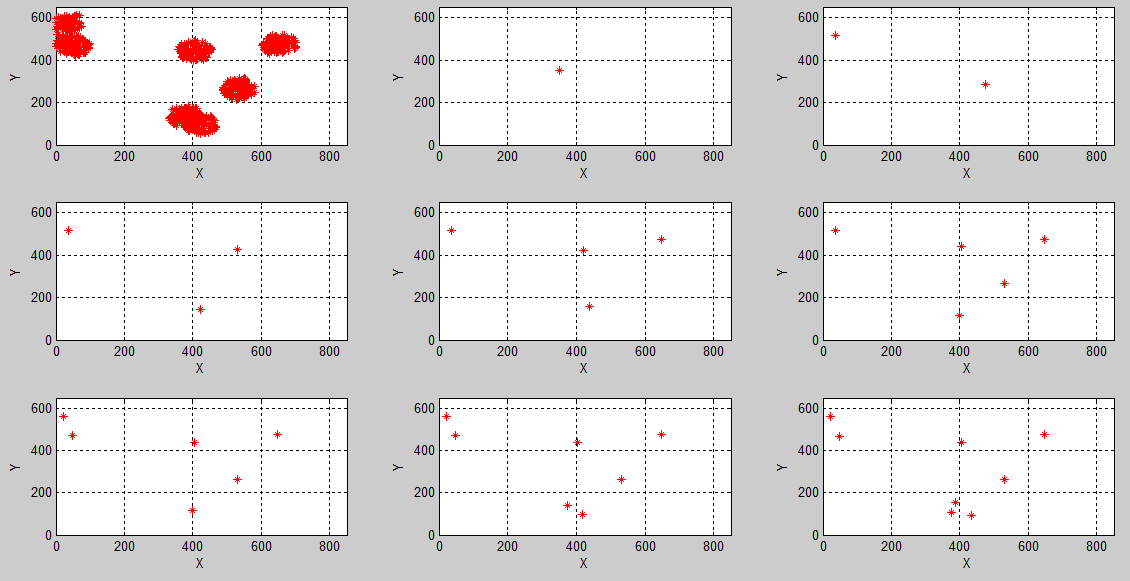
\includegraphics[width=5in]{GDataPlot11.png}
\caption{$(a)$ presents all observation points for k-means; altering the number of clusters, $K$, from 1 to 8, which are presented in $(b)-(i)$.}
\label{fig:plusCluster}
\end{figure}


\subsection{SLINK Clustering}
\label{sec:SLINK}
As described previously, for a certain time frame it is difficult to determine the exact number of clusters needed. We require an algorithm that can automatically determine the number of clusters. SLINK~\cite{sibson1973slink} is an algorithm that solves this problem. It treats each observation as a cluster initially and merges pairs of clusters in each iteration. In our experiment, we use the Euclidean distance as the distance metric and set up a threshold $T$ to stop merging clusters if the distance is larger. Since we know the exact size, $R$, of each cluster, we compare the results produced by different thresholds, $R/2$, $R$, and $2R$.  As shown in Fig.~\ref{fig:SLINKCluster}, different threshold values change the total number of clusters. A large threshold value, (d), yields only 4 centroids, while for lower threshold values the number of centroids increases. We notice that a threshold close to $R$ provides the best result.

%It is an agglomerative clustering algorithm, where each observation starts in its own cluster, and pairs of clusters are merged in each iteration. Therefore, in this approach, we would not need to care about the number of clusters we need to find in each time frame,  SLINK~\cite{sibson1973slink} is one of the efficient agglomerative clustering algorithm. In this approach, we use the Euclidean distance as the distance metric for the clustering. 
%In a fuzzy clustering algorithm, each point belongs to every cluster with a weight between 0 and 1, where 0 means the point does not belong and 1 means the point does completely belong to one cluster. Thus, clusters are treated as 'fuzzy sets', where a fuzzy set is a set in which an object belongs to any set with weight between 0 and 1. In a fuzzy clustering algorithm, each point belongs to every cluster with a weight between 0 and 1, where 0 means the point does not belong and 1 means the point does belong in the cluster. Thus, clusters are treated as `fuzzy sets'. A fuzzy set is a set in which an object belongs to any set with weight between 0 and 1. In fuzzy clustering an additional constraint may be imposed that the sum of the weights for each object must equal 1. This approach is appropriate in our setting since data points may be close to more than one cluster. 
%
\begin{figure}[h!]
\centering
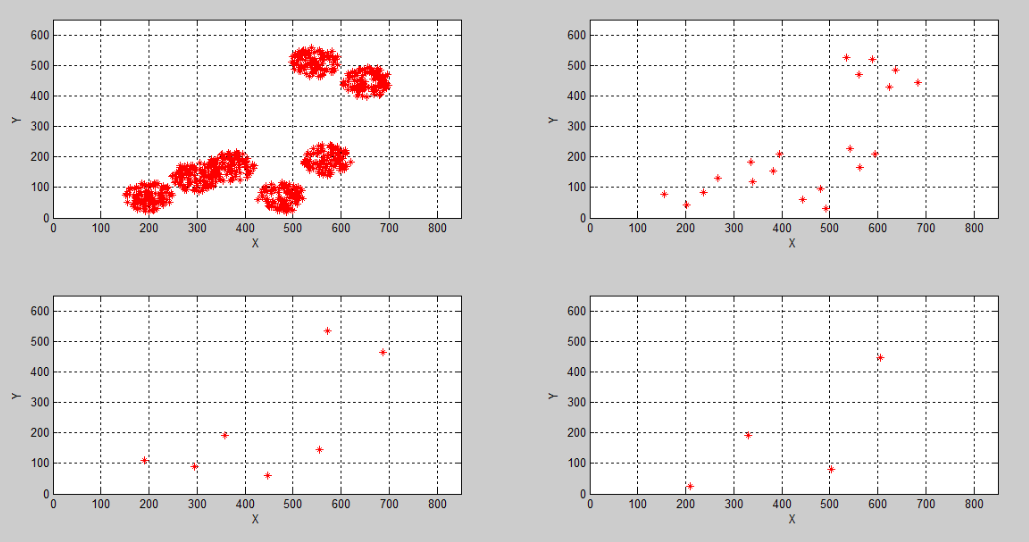
\includegraphics[width=5.5in]{GDataPlot6.png}
\caption{$(a)$ present all observation points for SLINK, $(b)$ presents the clusters found by set threshold $T=R/2$, $(c)$ presents the clusters found by set threshold $T=R$, $(d)$ present the clusters found by set threshold $T=2R$, where $R$ is the actual radius we used to generate these observations.}
\label{fig:SLINKCluster}
\end{figure}

\subsection{Hybrid Clustering}
Our goal is to find at most $N$ disks to cover all points at each time step, where $N$ is the number of ants, and maximizes the number of disjoint disks. In this case, we implement a hybrid clustering algorithm that uses both k-means++ and SLINK clustering. We use SLINK to determine the value $K$, where $K \leq N$, disks which cover all data points. We initially place $K=N$ group centroids into the space using the k-means++ algorithm. We then compare the Euclidean distance between two centroids. If the distance between any pair of centroids is closer than the threshold, we merge these two clusters. This reduces the total number of clusters from $K$ to $K-1$. We repeat this step until we cannot merge anymore clusters. Since we use the k-means++ algorithm to cluster our observations, the solution is guaranteed to be O(log $k$), competitive with the optimal k-means solution. In our experiment, we fixed the initial $K$ value to 8 and alter the threshold $T$. From Fig.~\ref{fig:bothCluster}, we see that the cluster merging process reduces the number of clusters $K$. Although different thresholds may still produce different results, as described in section~\ref{sec:SLINK}, we can set our threshold closer to the actual size of the observation clusters, which can be estimated initially, and thus avoid the threshold problem.

\begin{figure}[h!]
\centering
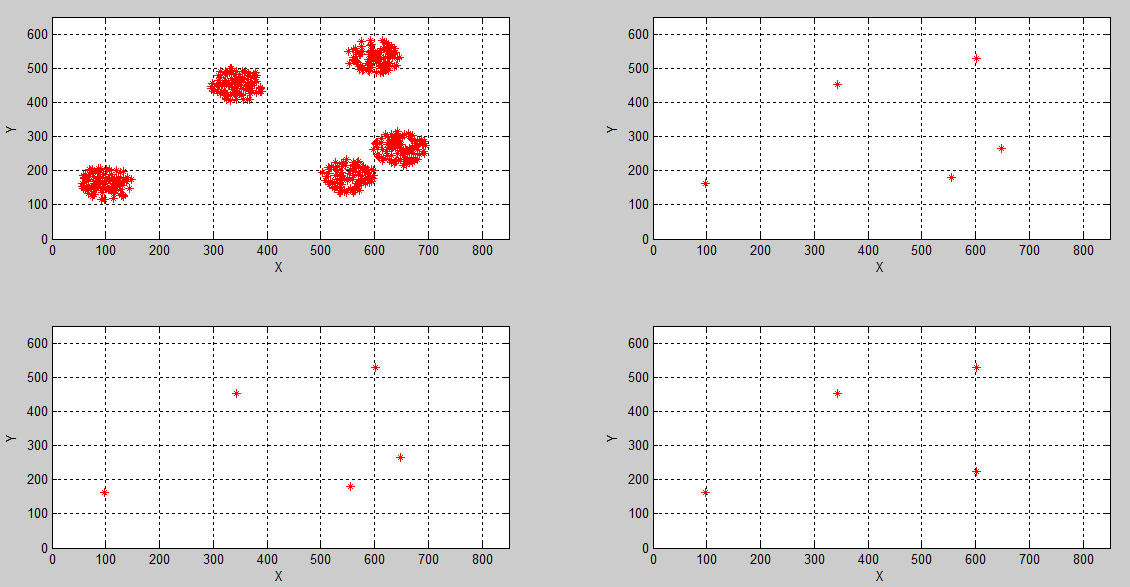
\includegraphics[width=5.5in]{GDataPlot12.png}
\caption{$(a)$ present all observation points for our hybrid algorithm. We set the initial $K$ value to 8: $(b)$ presents the clusters found by set threshold $T=R/2$, $(c)$ presents the clusters found by set threshold $T=R$, $(d)$ present the clusters found by set threshold $T=2R$, where $R$ is the actual range we used to generate these clusters.}
\label{fig:bothCluster}
\end{figure}

\section{Collecting and Generating Data}
In order to test the accuracy of the global approach we must first create a trajectory graph, $G$. We do this in two ways. The first uses simulated data, ie. simulated ant trajectories, and the second uses collected data. 

\subsection{Dataset}
We use a video with about 10,000 frames recorded at 30 frames per second of a {\it Temnothorax rugatulus} ant colony. In this video, ants are painted individually in order to identify them more easily. An automated multi-target system has been used to analyze the ant paths. A ground truth trajectory has been created by manually examining and correcting the automated trajectory. We use this ground truth to evaluate our algorithm. \\
In this data set there are 252 users generating trajectories for 50 ants. Each ant has 2-8 trajectories. We construct the intersection graph $G$ and apply the global greedy algorithm to build the representative trajectories. 

\subsection{Random Graph Generator}

Since intersections are the primary source of error when tracking ants, we randomly generate ant paths but force one intersection at every time step. We do this in order to test the global greedy algorithm on data with many intersections. \\
The forced-intersection algorithm is written in Matlab. It takes in the number of ants, the number of time frames, the dimensions of the space and the maximum displacement. The output is a text file with the x-coordinate and the y-coordinate for at each time frame for each ant. The path is generated using a 3D random walk. Intersections are forced by selecting an ant at random at each time step, then finding the nearest neighboring ant and determining an intermediate point at which they will meet. We set the x and y coordinates of the two ants accordingly then generate the coordinates for the remaining ants. In this algorithm, ants are equally likely to move up, down, left, right  or diagonally but are more likely to remain in their previous position. We generate 3 data sets using this algorithm each with 7 ants, 50 time frames, with a maximum displacement of 50 units. \\

\begin{figure}[h!]
\centering
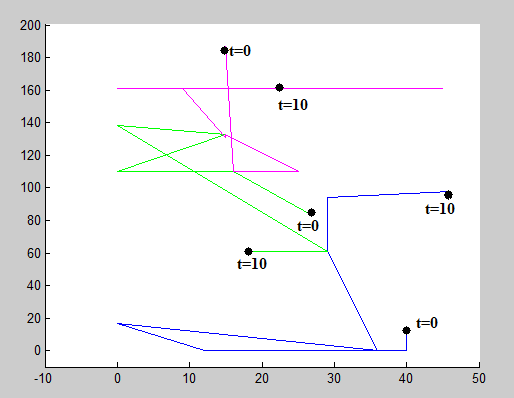
\includegraphics[width=4.5in]{GDataPlot3.png}
\caption{Three randomly generated ant paths for 10 time steps}
\label{fig:antPath}
\end{figure}


\subsection{Generating User Data}
Once the underlying graph is generated, we simulate user data. This algorithm takes in the text files with the generated ant paths and outputs text files with simulated trajectories of 100 users. Each output path represents a user tracking an ant in our base map. To generate this data we assume users always start at the correct point and users will only switch from one path to another when there is an intersection. When an intersection occurs, the user will switch paths with some fixed probability, the default is 0.25; a mistake will occur with probability 0.25 at each intersection point. We generate user data by randomly selecting x and y coordinates within a specified range of the true base map data, the default range is 20 units. We test error probabilities 0.01, 0.05, 0.10, 0.25. See Fig. \ref{fig:antData}.\\

\begin{figure}[h!]
\centering
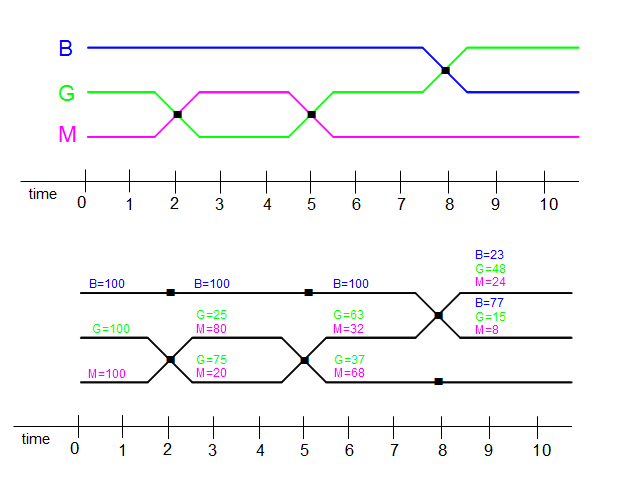
\includegraphics[width=4.5in]{GDataPlot4.png}
\caption{Trajectory graph for generated ant paths and simulated user data}
\label{fig:antData}
\end{figure}




\section{Greedy Algorithm}
We describe a heuristic for extracting representative trajectories from a collection of trajectories using a global greedy algorithm. We pick an ant at random and begin at its starting vertex in the global graph $G$. Each edge is weighted by the number of users who tracked that ant across that particular edge. We add an edge to the representative path if it has the maximum weight for that ant. We continue extending the representative path until the last time step is reached. We then remove these edges from $G$ and repeat the process. This continues until all $k$ representative trajectories have been determined. Since ants are chosen at random, we repeat this process and chose the set of representative trajectories with the highest weight over all trajectories.



 
%
%\section{Preliminary Statistical Analysis}
%We run the preliminary analysis on the same data set used in \cite{Joy12}. They used a video with about 10,000 frames recorded at 30 frames per second of a {\it Temnothorax rugatulus} ant colony. For this video only 5 ants were tracked although there were more than 5 ants present. We look at the standard deviation of each observed point to the ground truth, if the standard deviation falls below a specified threshold based on the average length in pixels of an ant, then the observation is considered to be exact. The result of this analysis demonstrate that the observations are reliable and that we do not need to introduce any considerations to reduce observational error. Ant44 was tracked by 8 users. After time frame 101, however, one user's standard deviation increased significantly. When cross-referencing the orginal data file it was clear this user was now tracking a stationary ant, whose path did not match any of the other 7 users. Once this outlying path was eliminated from the data, the standard deviation dropped below the threshold.\\
%This interesting event with Ant44 highlights several aspects of this statistical analysis. First, given that the standard deviation of the observed paths is quite low, it easy to determine when a user begins tracking another ant and which user begins to do so. This means it is easy to identify and eliminate this path from the data set for the specific ant. In addition, if we have a complete trajectory graph, we can cross reference this graph in order to determine which ant the outlying path could belong to. For example, for Ant44 one user began to deviate after frame 101, using this we can reference the global trajectory graph and determine which ant crossed paths with Ant44 between frames 101 and 201, then see if the deviant path matches the path of this other ant. If so, we can add this path to the data set for this ant instead. Thus eliminating this path from one data set while using it in another more appropriate data set. If this method is used, it is important that data is collected for every ant in the frame and the trajectory graph is compete, otherwise, it is not possible to detemine if the deviant path belongs to another ant.


\section{Experiments}
We analyze the performance of the global greedy algorithm on two sets of data. The first is using the citizen scientist method on a video of the {\it Temnothorax rugatulus} ant colony. We collect data from 252 users. We compare to the automated solution. The second is simulated trajectories using the forced-intersection algorithm. We generate 3 data sets using this algorithm each with 7 ants, 50 time frames, with a maximum displacement of 50 units. We vary the probability of error, testing 0.01, 0.05, 0.10 and 0.25. We also vary the clustering threshold, testing $R=10,20,40$. We calculate the variance of the representative trajectories from the true ant paths. We also compare the variance of the global greedy algorithm to the Homotopy Median algorithm. Finally we compare the variance of the homotopy median algorithm to the maximum, minimum and average variance for the global greedy algorithm

\section{Results and Discussion}
We compute the representative trajectories for each ant using the global greedy algorithm then compare to either the automated trajectory (for the collected data) or the true trajectory (for the generated data). We measure the average variance of the distance between pairs of points of the computed and true trajectories. \\

\begin{figure}[h!]
\centering
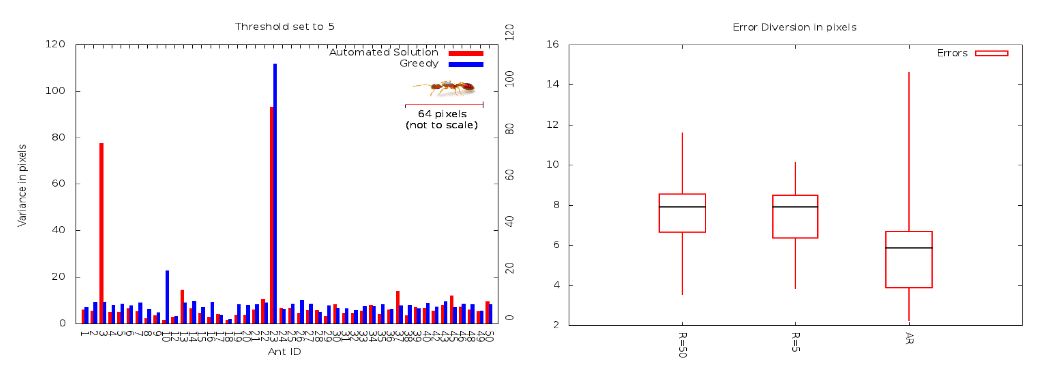
\includegraphics[width=7in]{range5Div.png}
\caption{Average variance in pixels of global greedy vs. automated solution with threshold set to 5 pixels. Average error for R=5, R=50 and automated solution}
\label{fig:real}
\end{figure}

We can see that for the collected data the global greedy algorithm performs similarly to the automated solution. The average variance of both algorithms generally remains below 20 pixels for both thresholds $R=5$ and $R=50$. The box and whisker plot in Figure \ref{fig:error} demonstrates that although the average error for the automated solution is slightly less, about 6 pixels, the variance is quite large, about 13 pixels. For the global greedy algorithm, the average error is about 8 but the variance is only 8 for $R=50$ and 6 for $R=5$.

%\begin{figure}[h!]
%\centering
%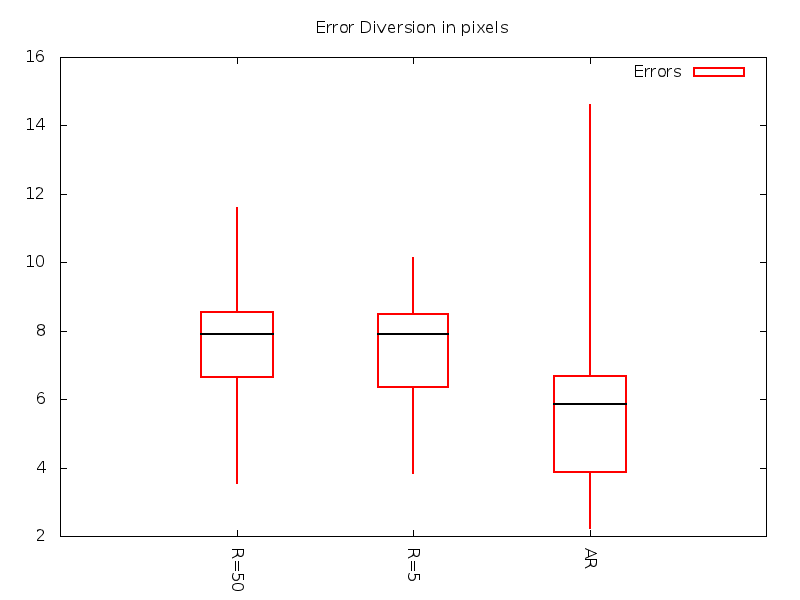
\includegraphics[width=3.5in]{div.png}
%\caption{Average error for R=5, R=50 and automated solution}
%\label{fig:error}
%\end{figure}

For the generated data we plot the average variance for $R = 10,20,40$. Again this is the average variance of each point from the true path. We notice that the variance for all three data sets is between 20-30 pixels. We can see that in general the lower threshold value has a smaller variance but that this is not always the case. For ant 1 in data set 2, the lower threshold (in blue) has a significantly higher variance than the larger threshold values. While for ant 5 in the same data set the lower threshold has a much smaller variance than the other two. Although we can not determine from these experiments the ideal threshold value it is clear that the threshold plays an important role in determining the variance of the representative trajectory. 
\begin{figure}[h!]
\centering
\includegraphics[width=6in]{GDataPLot1.png}
\caption{Average variance for $R=10,20,40$ pixels for Data Set 1 and Data Set 2}
\label{fig:error}
\end{figure}

\begin{figure}[h!]
\centering
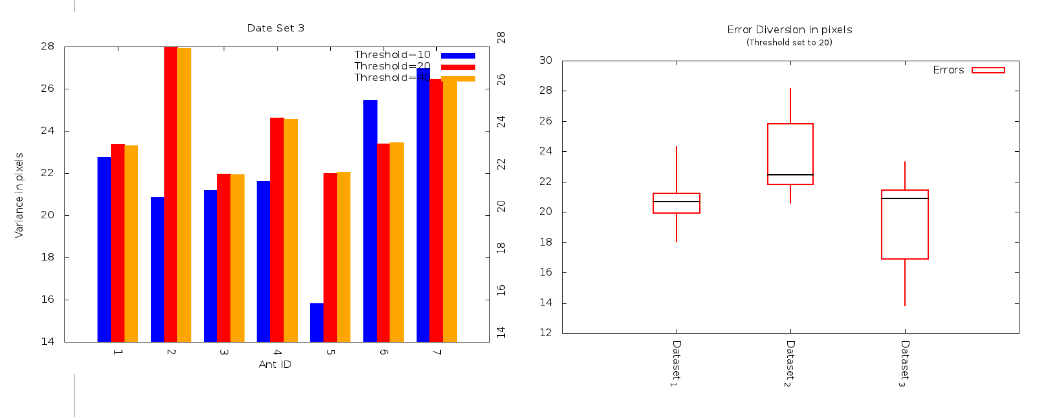
\includegraphics[width=6in]{GDataPlot2.png}
\caption{Average variance for $R=10,20,40$ pixels for Data Set 3 and average error plot}
\label{fig:error}
\end{figure}
We then examine the effect of the probability of  user error on the average variance of the representative path. See Fig. \ref{fig:prob}. Here we vary the probability that a user mistakenly switches paths, we test 1\%, 5\%, 10\% and 25\% probability of error. For each error probability we also vary the clustering threshold from $R=10$ to $R=20$ to $R=40$. 

\begin{figure}[h!]
\centering
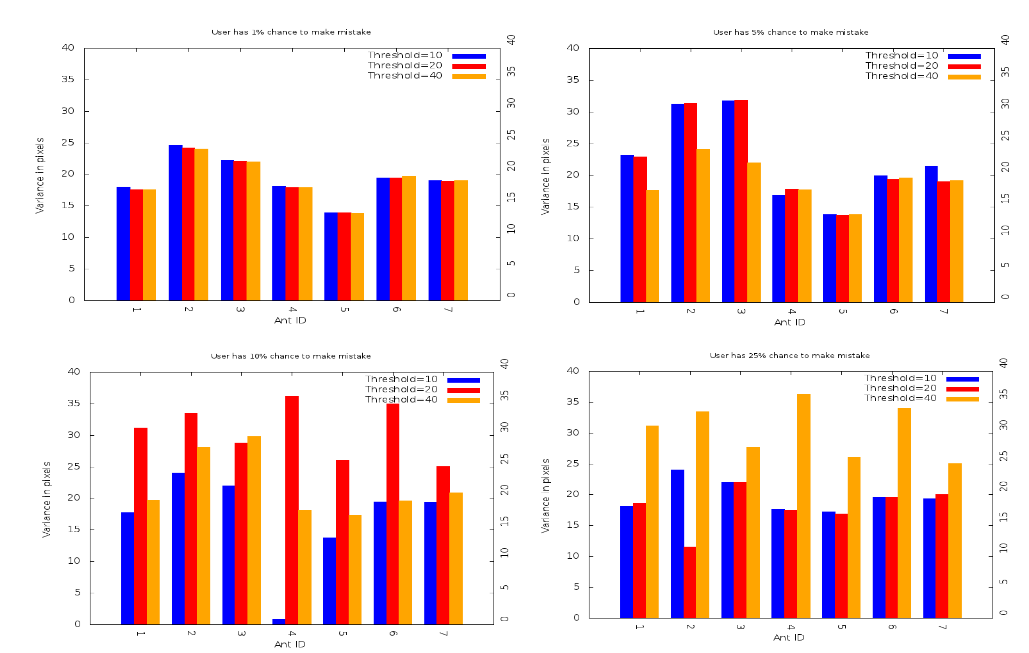
\includegraphics[width=6in]{GDataPlot8.png}
\caption{Data Set 2}
\label{fig:prob}
\end{figure}

Note that at 1\% probability of error the clustering threshold has little effect of the average variance of the representative path. The variance for all thresholds remains between 15-20 pixels. When the error is increased to 5\% we notice that the larger clustering threshold has a lower variance and the variance is now between 15-33 pixels. In the case of 10\% user error, the 20 pixel clustering threshold has the largest variance for 6 of the 7 ant paths and the variance is between 2-35 pixels. Finally in the case of 25\% user error, the 40 pixel threshold has the largest variance for all 7 ants and the variance is between 10-35 pixels. The relationship between probability of user error and clustering threshold is interesting to note. There is not one single threshold value that is lowest across all probabilities.\\
Examining the data in a slightly different way, Fig \ref{fig:thresh}, we can see that each clustering threshold minimizes the variance for a different probability of error. For the threshold value of 10, we see that the variance is low when the probability of error is 1\%, 10\%, and 25\%. But is much higher when the probability of error is 5\%. When the threshold is 20, the variance is much larger when the probability of error is 5\% and 10\%. When the clustering threshold is 40, the variance is larger when the probability of error is 10\% and 25\%. We can conclude that if there is a low probability of error  about 1\% then any threshold will produce a representative path with low variance. If the probability of error is about 5\%  then a high threshold, about 40, will yield a path with low variance. If the probability of error is about 10\% then a low threshold, about 10, results in a path with low variance and if the probability of error is 25\% then a threshold value between 10-20 will yield a path with low variance.  

\begin{figure}[h!]
\centering
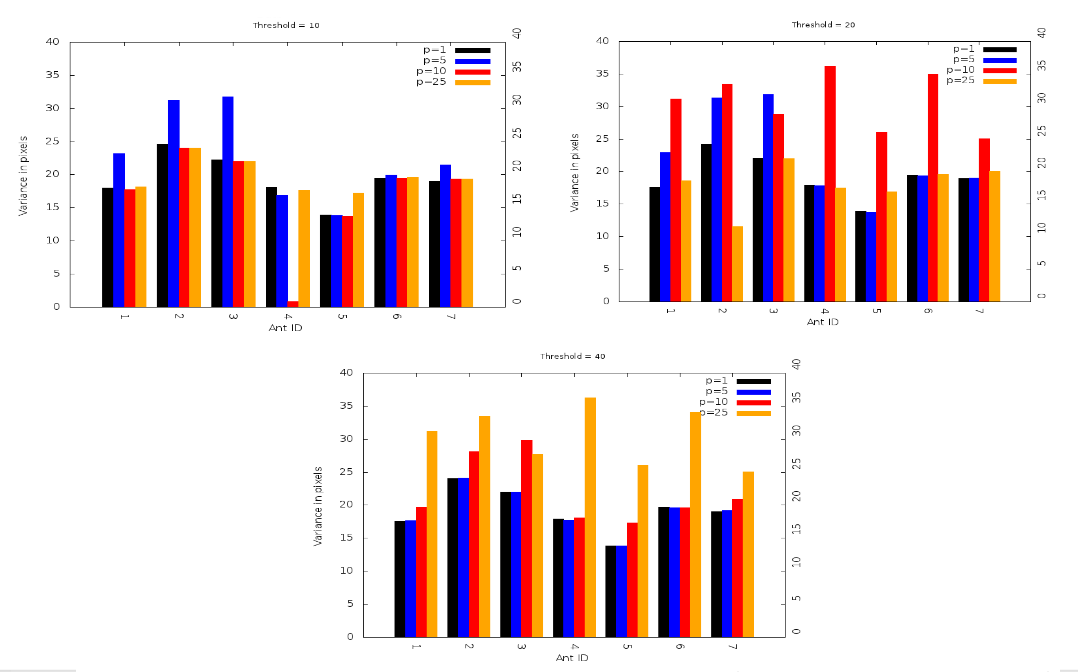
\includegraphics[width=6.5in]{GDataPlot9.png}
\caption{Data Set 2}
\label{fig:thresh}
\end{figure}

We can further observe this relationship between probability of user error and clustering threshold using the box and whisker plot in Fig. \ref{fig:whisker}. At 5\% user error the average error for all data sets across all threshold values is between 20-25 pixels. All errors lie between 15-35 pixels. At 10\% user error, however, the average error for Data Sets 2 and 3 fluctuate depending on the clustering threshold. The minimum error is 2 pixels, while the maximum error is 35 pixels. It is interesting to note that Data Set 1 seems to be invariant with respect to both the clustering threshold and the probability of user error. In fact, even when the user error is 25\% the box and whisker plot remains unchanged. It is still unclear what caused this result.   

\begin{figure}[h!]
\centering
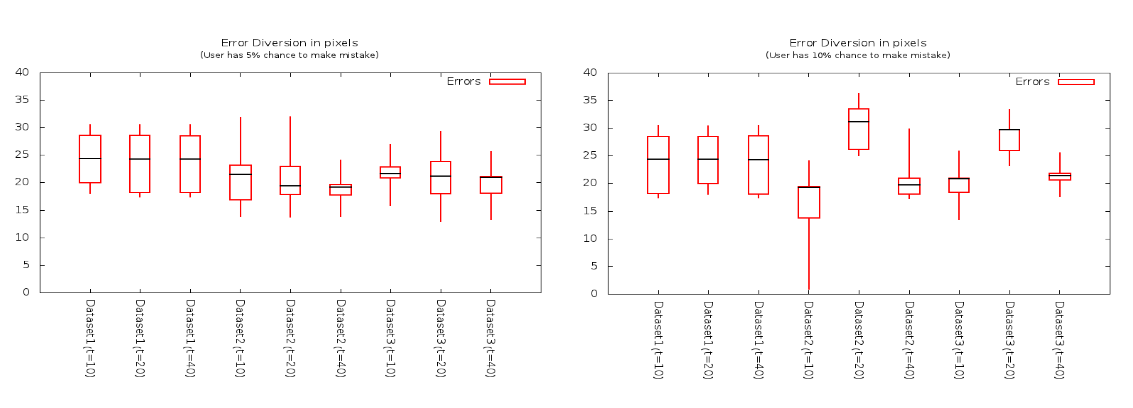
\includegraphics[width=6in]{GDataPlot10.png}
\caption{Average error for probability of user error 5\% and 10\%}
\label{fig:whisker}
\end{figure}

We compare the variance of the global greedy algorithm to the local homotopy median algorithm. See Fig. \ref{fig:compare}. We use Data Set 1 and compare the average variance of both algorithms. We can see the variance for the local homotopy algorithm is between 40 and 90 pixels while the global greedy algorithm is around 20 pixels.

\begin{figure}[h!]
\centering
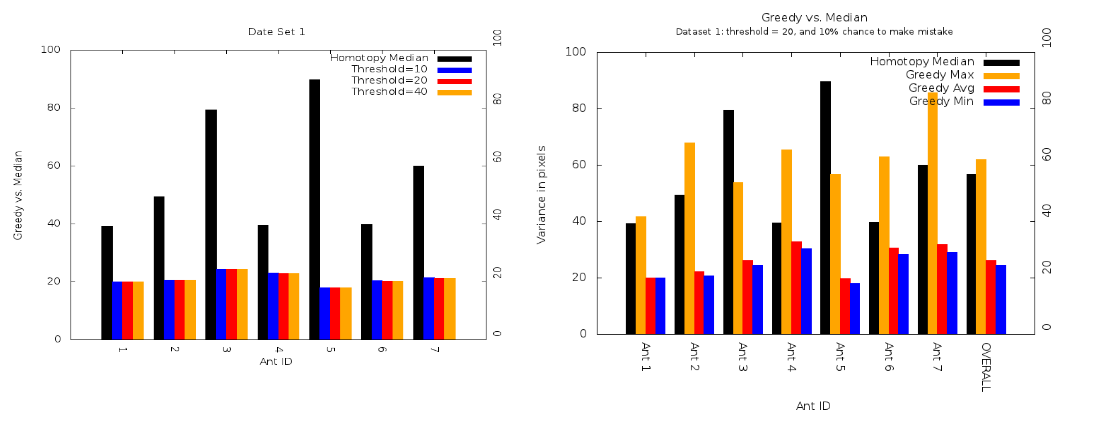
\includegraphics[width=6in]{compare.png}
\caption{Global greedy vs. local homotopy median}
\label{fig:compare}
\end{figure}

Since the global greedy algorithm is a randomized algorithm we compare the maximum, minimum and average variance of the global algorithm to the variance of the homotopy median algorithm. See Fig. \ref{fig:compare}.  We see that in the best and average cases, the global greedy algorithm has a lower variance than the local homotopy algorithm. In the worst case, however, it is no better than the local algorithm. More plots can be found in the appendix.

%\begin{figure}[h!]
%\centering
%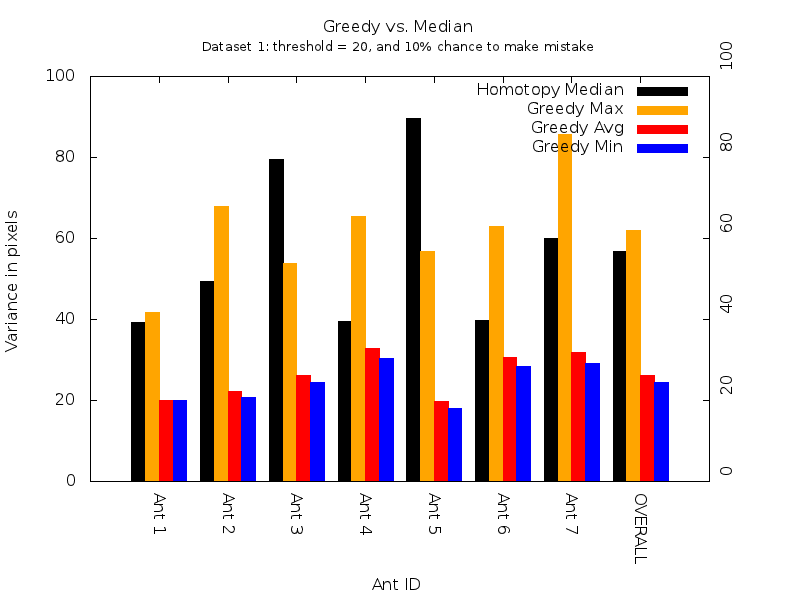
\includegraphics[width=5in]{random_cmp.png}
%\caption{Global greedy vs. local homotopy median}
%\label{fig:compRand}
%\end{figure}

\section{Conclusions and Future Work}
We explored a global greedy algorithm for extracting representative trajectories from a large number of input trajectories. When analyzing user data collected by `citizen scientists' we found that the global greedy algorithm was comparable to the automated solution. We demonstrated that the global greedy algorithm is sensitive to changes in the user probability of error and the clustering threshold. We found that the global greedy algorithm out-performs the local homotopy median algorithm in both the best and the average cases, but not in the worst case. \\
It would be interesting to continue exploring the effect of user error and the clustering threshold on representative trajectories, especially considering the results of Data Set 1. It would also be interesting to determine the average probability of error from user data. We test a range of probabilities here but have no analysis to indicate what the observed value actually is. \\
We also hope to perform a similar analysis on other global algorithms to see the sensitivity of other algorithms to the probability of error and the clustering threshold. 

\newpage

\section{Appendix}

\begin{figure}[h!]
\centering
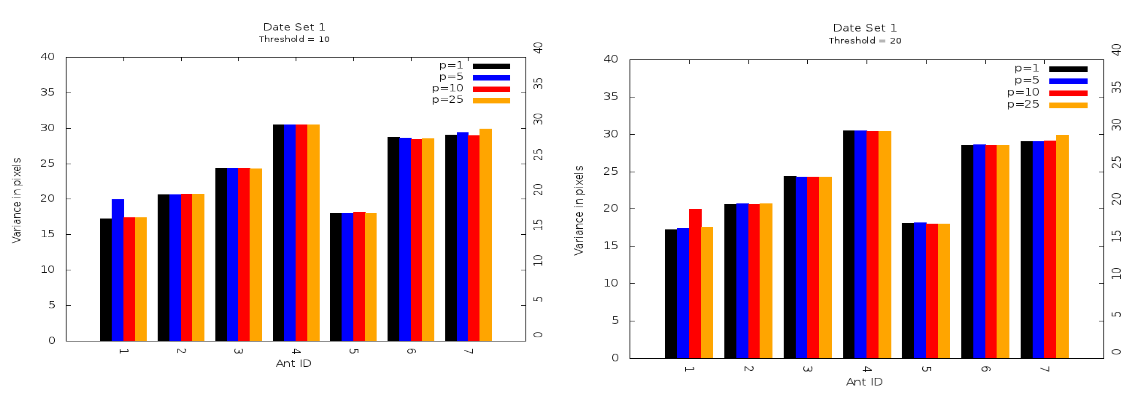
\includegraphics[width=6in]{GDataPlot13.png}
\caption{Data Set 1 with threshold $R=10, 20$}
\label{fig:DS1}
\end{figure}

\begin{figure}[h!]
\centering
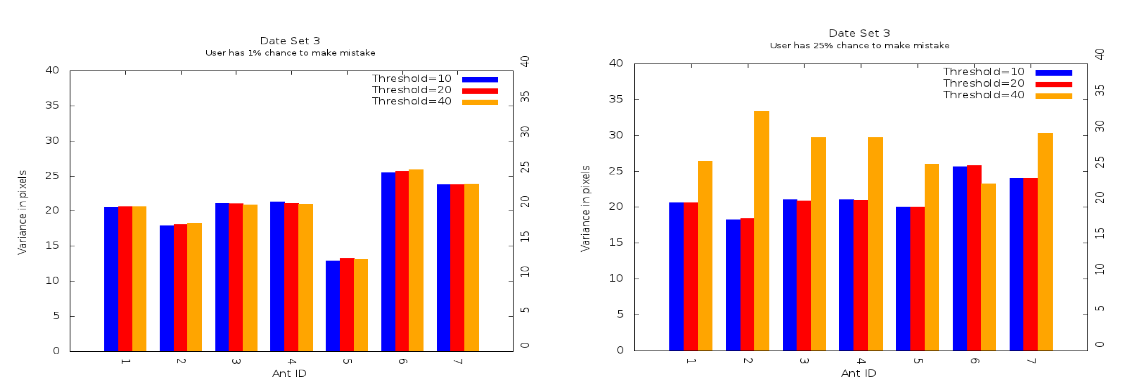
\includegraphics[width=6in]{GDataPlot14.png}
\caption{Data Set 3 with probability of error 1\% and 25\%}
\label{fig:DS3P}
\end{figure}

\begin{figure}[h!]
\centering
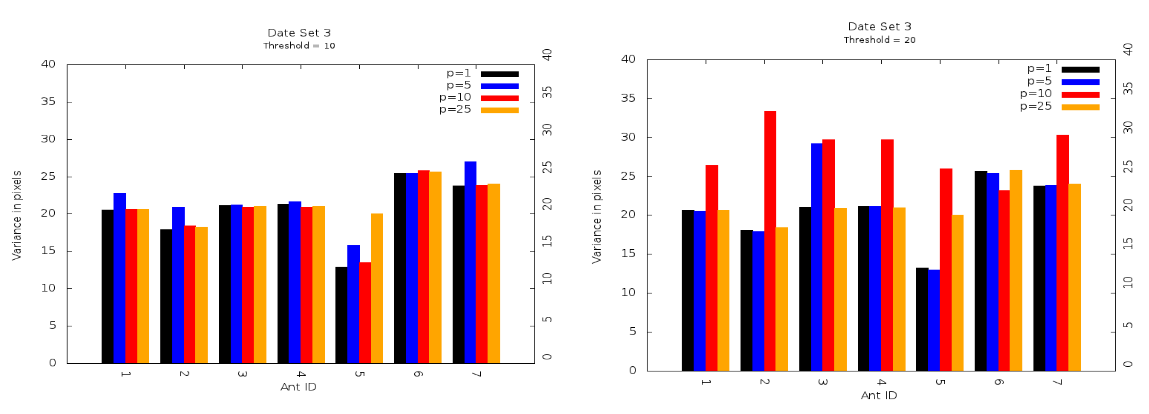
\includegraphics[width=6in]{GDataPlot15.png}
\caption{Data Set 3 with threshold $R=10,20$}
\label{fig:DS3R}
\end{figure}


\begin{figure}[h!]
\centering
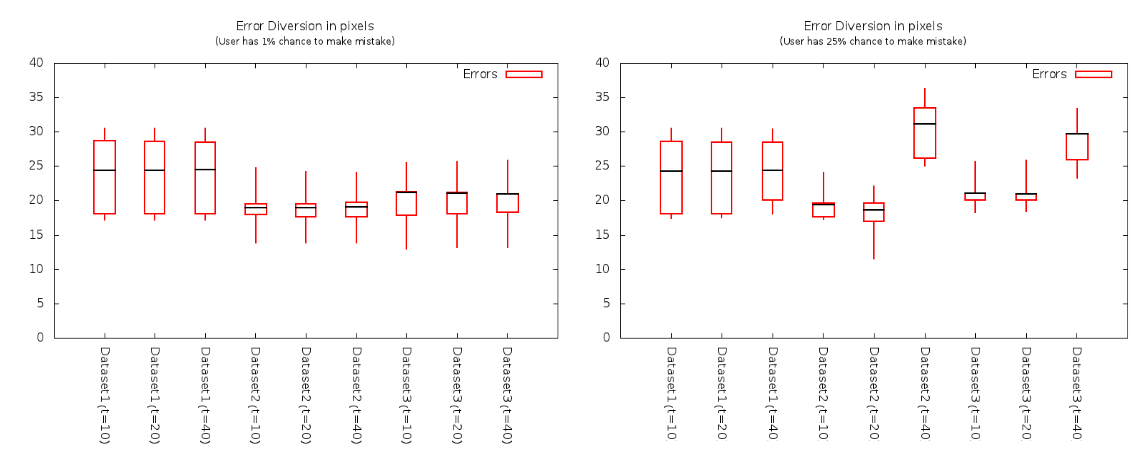
\includegraphics[width=6in]{GDataPlot16.png}
\caption{Error for 1\% probability and 25\% probability}
\label{fig:error1}
\end{figure}

\begin{figure}[h!]
\centering
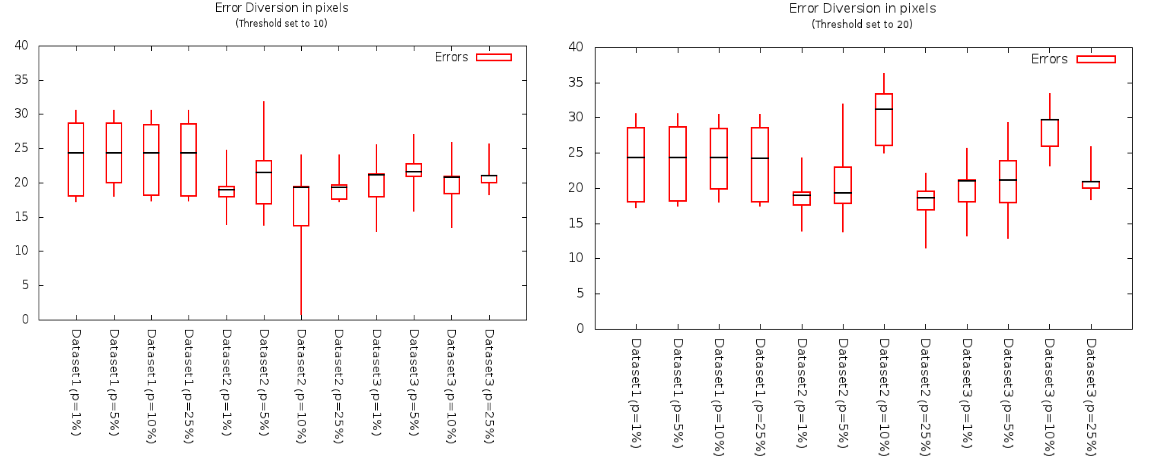
\includegraphics[width=6in]{GDataPlot17.png}
\caption{Error for threshold $R=10,20$}
\label{fig:error2}
\end{figure}

\begin{figure}[h!]
\centering
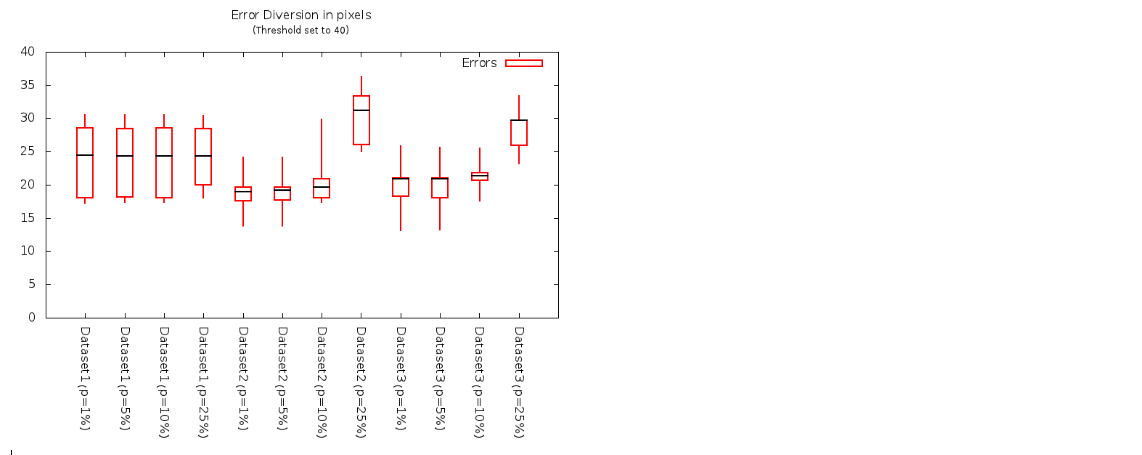
\includegraphics[width=6in]{GDataPlot18.png}
\caption{Error for threshold $R=40$}
\label{fig:error3}
\end{figure}

\newpage
%Explore parameters, shot-gun sequencing to glue segments together, other global algorithms, find optimal radius of clusters, randomized algorithm analysis\\




\bibliography{hayley}
\bibliographystyle{plain}

\end{document}

% The goal of this project is to create an algorithm that computes a network flow as described above such that each path is `feasible' and `optimal'.  We will begin by exploring a simple Greedy algorithm then the min-cost flow problem and, as suggested by \cite{Joy12}, implement an algorithm that finds the optimal path for ant $A$ and removes these paths, then ant $B$, removes these paths, etc. \\
%
%
%
%\begin{center}\begin{tabular}{|c|c|c|c|c|}
%	\hline Algorithm & local/global & time & implemented?& Who? \\
%	\hline Frechet & local & No & Yes & \cite{Joy12} \\
%	\hline Median & local & No & Yes & \cite{Joy12} \\
%	\hline MC Basic & global & Yes & pilot test & Paul, Jasmin \\
%	\hline Lin. Prog. & global & Yes & up to 3 & Sergei\\
%	\hline k-Clustering & global & Yes & in prog & Yunhao\\
%	\hline Shotgun & global & Yes & No & Paul, Jasmin\\
%	\hline
%	\end{tabular}\end{center}
%
%
%\indent In order to determine how far the paths we generate are from the `ground truth' we will use least squares distance and Frechet distance. If needed, we may develop a new metric specific to the data in order to evaluate the distance between paths.\\
%\indent If time permits we will explore the effectiveness and efficiency of various validation schemes.

%\section{Shotgun Method}
%\indent We propose an alternative approach based on shotgun sequencing in DNA \cite{Anson10}. We notice that over time users tend to lose interest in tracing the ant path. This results in more errors in the data as time increases. We take advantage of the initial, more accurate portions of the path by initializing path-tracing at different times. For example, suppose we wish to track ant $A$. We ask $n$ users to track ant $A$, where each user begins tracking at a different time $\{t_1,...,t_n\}$. Taking these $n$ paths we will then identify the portions that are at the same time step. We can then `glue' the paths together at these matching portions and ultimately, determine a resulting path that is a continuous curve from start time to end time.\\
%\indent In the implementation of this approach there are three factors to test: the partition of initial observation times, the distribution of observation lengths, and the maximum observation time before the observer begins to lose interest. In the initial implementation, the starting times will be equally spaced- in other words, the partition will be uniform. We can begin by requiring that all observers trace the path for a fixed amount of time. \\
%\subsection{Algorithm}
%This method is based on DNA shot-gun sequencing, a method used to sequence large amounts of genetic material, the entire human genome, for example. The premise of the method is that a long fragment of genetic code can be sequenced by sequencing shorter randomly selected segments that overlap then `glueing' these segments together at the overlaping regions. This method decreases the error since mistakes are less likely to occur when sequencing shorter segments. Similarly, when tracking ants, the user is more likely to lose interest and make a mistake the longer they trace a trajectory. Taking this into consideration, we propose the shot-gun method for determining ant trajectories. \\
%\indent We begin by describing the data collection phase of the method. Previoulsy, users were asked to track a specific ant for exactly the same fragment of video. In this method, each observation will be initialized at a random time and ultimately the length of each fragment will also be randomly distributed. A new segment will be chosen until every time has been tracked at least 5 times. These segments will then be pieced together according to the time stamp. There will be five different data points associated to each time step. If all are within 17 pixels, an average will be taken and this will be a point on the representative trajectory. If there is an outlier, we determine if this was at the start of a trace or the end of a trace and weight this value appropriately or we use the trajectory graph to determine if an error occured at a crossing.

%Given the number of ants in the frame and the `ground truth' trajectory for each ant we beign by selecting an ant at random using a uniformly distributed discrete random variable. We then select a random time/place pair from the `ground truth' data for this ant. The game will be initialized at this time and place. We begin by having users track for a fixed amount of time then we run a second round of experiments where users track for a randomly distributed amount of time. \\
%\indent We must ensure that each point in the trajectory is traced sufficiently many times in order to minimize the error. We calculate this number using the orginal data set used in the local trajectory analysis. We use the standard deviation of  the distance from each observed point to the ground truth.
%%Let $X_{i}^{a}$ be the `ground truth' position of ant $a$ at time $i$. Let $\{Y_{1,i}, ...Y_{n,i}\}$ be the position of ant $a$ at time $i$ as observed by $n$ users. We determine the standard deviation $ S = \sqrt{\frac{1}{n}\sum\limits_{j =1}^n {(Y_{j,i}-X_i^a)^2}}$.
% For example, for Ant5 six users collected data. We look at the following frames \{1,101,201,301...,3301\}. For each user and each frame we compute the square of the Euclidean distance from the observed point to the ground truth. We then compute the average square distance across all users for each time frame. The square root of this number is the standard deviation. Since an ant is assumed to be 17 pixels long, we took a ball of radius $\frac{17}{2}$ as a threshold. If the standard deviation falls within this ball, we assume the observations to be exact. \\
%\indent We perform this analysis for Ant5, Ant6, Ant27, Ant36, and Ant44. For Ants 5,6,27, and 36, the standard deviation fell beneath the threshold for almost every time frame, in the few cases it did not, the deviation was less than 2 pixels. These results demonstrate that the observations are reliable and that we do not need to introduce any considerations to reduce observational error. Ant44 was tracked by 8 users. After time frame 101, however, one user's standard deviation increased significantly. When cross-referencing the orginal data file it was clear this user was now tracking a stationary ant, whose path did not match any of the other 7 users. Once this outlying path was eliminated from the data, the standard deviation dropped below the threshold. \\
%\indent This interesting event with Ant44 highlights several aspects of this statistical analysis. First, given that the standard deviation of the observed paths is quite low, it easy to determine when a user begins tracking another ant and which user begins to do so. This means it is easy to identify and eliminate this path from the data set for the specific ant. In addition, if we have a complete trajectory graph, we can cross reference this graph in order to determine which ant the outlying path could belong to. For example, for Ant44 we know one user began to deviate after frame 101, using this we can reference the graph and determine which ant crossed paths with Ant44 between frames 101 and 201, then see if the deviant path matches the path of this other ant. If so, we can add this path to the data set for this ant instead. Thus eliminating this path from one data set while using it in another more appropriate data set. If this method is used, It is important that dat is collected for every ant in the frame and the trajectory graph is compete, otherwise, it is not possible to detemine if the deviant path belongs to another ant. \\